\section{Validation}
\label{sec:Validation}
In order to have a valid result, we had to execute the application for each Garbage collection mechanism at least for 5 minutes.\\
PowerAPI generates an output file with the informations related to the execution (Process ID, duration, energy consumption\ldots)\\
An automatic script treats an output file was executed for each output file to generate a modified file with only the extraction of the value of energy consumption.\\
these modified files were passed to Gnuplot\cite{gnuplotOfficial} : a command-line program that can generate two -and three-dimensional plots of functions, data, and data fits.\cite{gnuplot}

\subsection{Results}
Using Gnuplot I was able to generate a graph representing the energy consumption for each Garbage collection in time:\\

\begin{figure}[H]
	\centering
	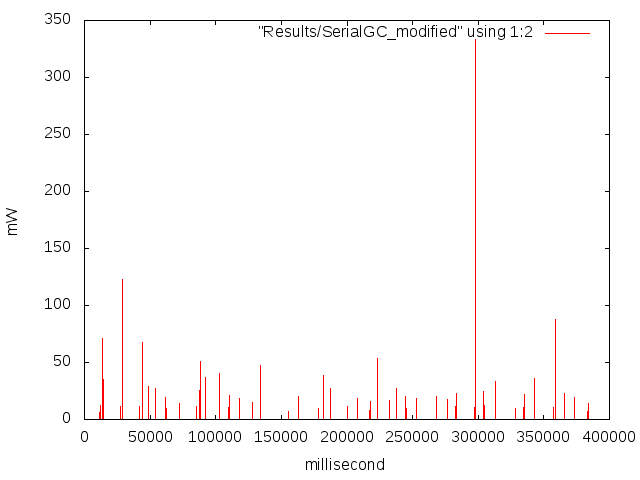
\includegraphics[width=12cm,keepaspectratio]{images/SerialGC.png}
	\caption{Serial Garbage collector}
\end{figure}

\begin{figure}[H]
	\centering
	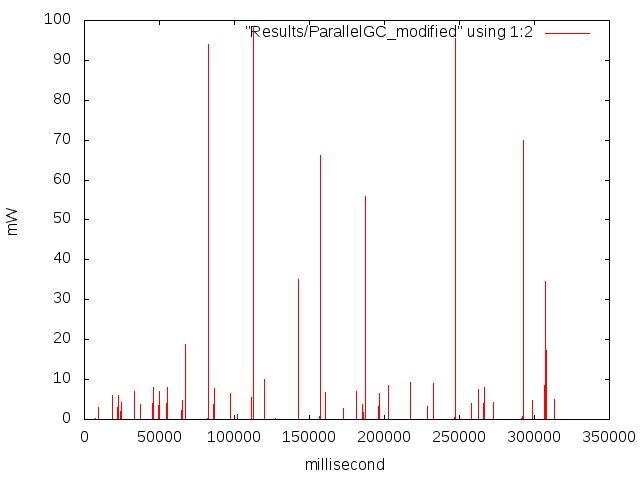
\includegraphics[width=12cm,keepaspectratio]{images/ParallelGC.png}
	\caption{Parallel Garbage collector}
\end{figure}

\begin{figure}[H]
	\centering
	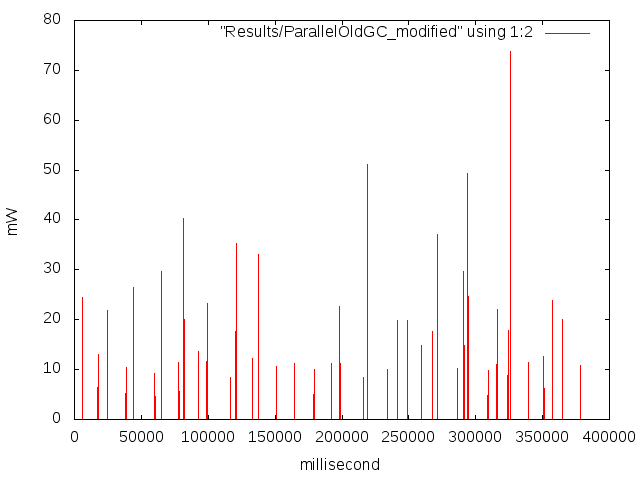
\includegraphics[width=12cm,keepaspectratio]{images/ParallelOldGC.png}
	\caption{ParallelOld Garbage collector}
\end{figure}

\begin{figure}[H]
	\centering
	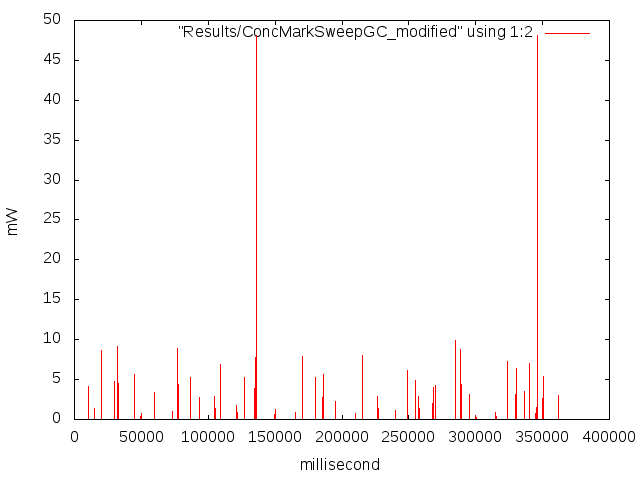
\includegraphics[width=12cm,keepaspectratio]{images/ConcMarkSweepGC.png}
	\caption{ConcMarkSweep Garbage collector}
\end{figure}

\begin{figure}[H]
	\centering
	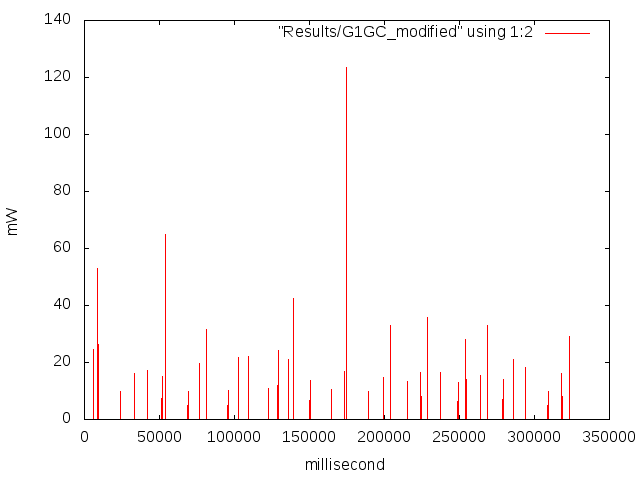
\includegraphics[width=12cm,keepaspectratio]{images/G1GC.png}
	\caption{G1 Garbage collector}
\end{figure}

As we can see from the graph presented above, the average consumption for Serial Garbage collector is around 34.7mW 
while the average consumption for Parallel is around  16.2mW and for ParallelOld is around 21.2mW.\\
For ConcMarkSweep Garbage collector the consumption is around 6.3mW while for G1 Garbage collector it is arround 24.1mW.\\
We Can conclude that Serial Garbage collector is the most consuming Garbage collector and ConcMarkSweep is the least consuming Garbage collector.\\
As we can see, none of the four Garbage collector consumes a lot of energy, so we can safely say that the choice of the garbage collector for a Java application won't play a significant role in determining the energy consumption of an application.